\documentclass{standalone}

\usepackage{amsmath}

\usepackage{tikz}
\usetikzlibrary{backgrounds}
\usetikzlibrary{positioning}
\usetikzlibrary{calc}
\usetikzlibrary{trees}									% for trees
\usetikzlibrary{shapes.multipart}

\usepackage{xcolor}
\definecolor{mygreen}{RGB}{0,128,0}


\begin{document}
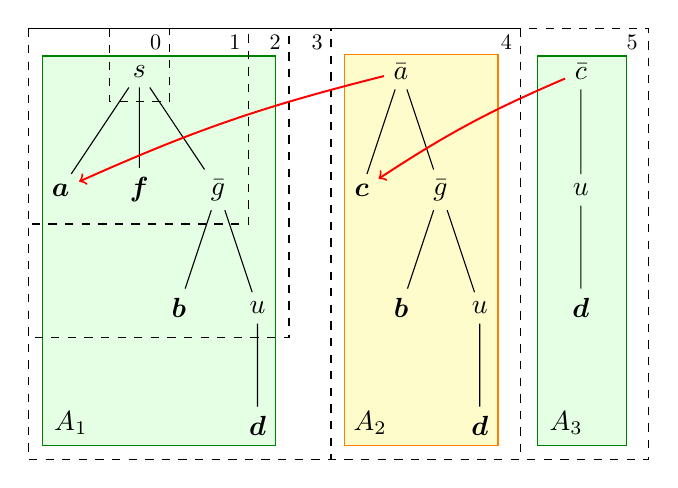
\begin{tikzpicture}

  
  
%P: First argument
\node (ps) {$s$}
child {node[xshift=0.5cm]  (pa) {$\boldsymbol{a}$}}
child {node (pf) {$\boldsymbol{f}$}}
child {node[xshift=-0.5cm]  (pxg) {$\bar{g}$}
    child {node[xshift=0.25cm]  (pb) {$\boldsymbol{b}$}}
    child {node[xshift=-0.25cm]  (pu) {$u$}
        child { node (pd2) {$\boldsymbol{d}$} }
    }  
};


\begin{pgfonlayer}{background}
    \filldraw [fill=green!20, fill opacity=0.5, draw=mygreen]
                    (ps.north -| pa.west)
        rectangle (pd2.south -| pd2.east);
        \node at ([shift={(-3pt,8pt)}]pd2.south -| pa.east) {$A_1$};
    \end{pgfonlayer}    


%O: second argument    
% %O:  Arg attacking A - 1		
\node[right = 2.9cm of ps] (pxa) {$\bar{a}$}
child {node[xshift=0.25cm]  (pxav) {$\boldsymbol{c}$}}
child {node[xshift=-0.25cm]  (pxaxg) {$\bar{g}$}
    child {node[xshift=0.25cm]  (pxab) {$\boldsymbol{b}$}}    
    child {node[xshift=-0.25cm]  (pxau) {$u$}
        child {node (pxad2) {$\boldsymbol{d}$}}
    }    
};

\begin{pgfonlayer}{background}
    \filldraw [fill=yellow!40, fill opacity=0.5, draw=orange]
                    (pxa.north -| pxav.west)
        rectangle (pxad2.south -| pxad2.east);
        \node at ([shift={(-3pt,8pt)}]pd2.south -| pxav.east) {$A_2$};
    \end{pgfonlayer}


%P: third argument    
% %O:  Arg attacking A - 1		
\node[right = 5.2cm of ps] (pxc) {$\bar{c}$}
child {node (pxcu) {$u$}
    child {node (pxcd) {$\boldsymbol{d}$}}    
};

\begin{pgfonlayer}{background}
    \filldraw [fill=green!20, fill opacity=0.5, draw=mygreen]
                    ([shift={(-10pt,0pt)}]ps.north -| pxc.west)
        rectangle ([shift={(10pt,0pt)}]pd2.south -| pxcd.east);
        \node at ([shift={(-11pt,8pt)}]pd2.south -| pxc.east) {$A_3$};
    \end{pgfonlayer}    

    

% Third argument
\begin{pgfonlayer}{background}
    \filldraw [fill=white, fill opacity=0, dashed]
    ([shift={(-5pt,10pt)}]ps.north -| pa.west)
    rectangle ([shift={(8pt,-5pt)}]pd2.south -| pxad2.east) ;
    \node [scale=0.8] at ([shift={(3pt,5pt)}]ps.north -| pxad2.east) {4};
\end{pgfonlayer} 






% Second argument
\begin{pgfonlayer}{background}
    \filldraw [fill=white, fill opacity=0, dashed]
    ([shift={(-5pt,10pt)}]ps.north -| pa.west)
    rectangle ([shift={(18pt,-5pt)}]pd2.south -| pxcd.east) ;
    \node [scale=0.8] at ([shift={(12pt,5pt)}]ps.north -| pxcd.east) {5};
\end{pgfonlayer} 


% First argument

\begin{pgfonlayer}{background}
    \filldraw [fill=white, fill opacity=0, dashed]
    ([shift={(-5pt,10pt)}]ps.north -| pa.west)
    rectangle ([shift={(20pt,-5pt)}]pd2.south -| pd2.east) ;
    \node [scale=0.8] at ([shift={(15pt,5pt)}]ps.north -| pd2.east) {3};
\end{pgfonlayer}  	


\begin{pgfonlayer}{background}
    \filldraw [fill=white, fill opacity=0, dashed]
    ([shift={(-5pt,10pt)}]ps.north -| pa.west)
    rectangle ([shift={(5pt,-5pt)}]pu.south -| pu.east) ;
    \node [scale=0.8] at ([shift={(0pt,5pt)}]ps.north -| pu.east) {2};
\end{pgfonlayer}  	


\begin{pgfonlayer}{background}
    \filldraw [fill=white, fill opacity=0, dashed]
    ([shift={(-5pt,10pt)}]ps.north -| pa.west)
    rectangle ([shift={(5pt,-5pt)}]pxg.south -| pxg.east) ;
    \node [scale=0.8] at ([shift={(0pt,5pt)}]ps.north -| pxg.east) {1};
\end{pgfonlayer}  	


\begin{pgfonlayer}{background}
    \filldraw [fill=white, fill opacity=0, dashed]
                  ([shift={(-5pt,10pt)}]ps.north -| ps.west)
        rectangle ([shift={(5pt,-5pt)}]ps.south -| ps.east);
        \node [scale=0.8] at ([shift={(0pt,5pt)}]ps.north east) {0};
    \end{pgfonlayer}


    







% \begin{pgfonlayer}{background}
% \filldraw [fill=yellow!40]
%               (xah.south -| xah.east)
%     rectangle (xa.north -| xae.west);
% \end{pgfonlayer}       

% %O: Arg attacking A - 2		    
% \node[right = 2cm of xa] (xa2) {$\bar{a}$}
% child {node (xa2e) {$\boldsymbol{e}$}}
% child {node (xa2v) {$v$}
%     child {node (xa2i) {$\boldsymbol{i}$}}    
% }; 

% \begin{pgfonlayer}{background}
% \filldraw [fill=yellow!40]
%               (xa2i.south -| xa2i.east)
%     rectangle (xa2.north -| xa2e.west);
% \end{pgfonlayer}           
    
% %O: Arg attacking A - 3				
% \node[right = 1.25cm of xa2] (xa3) {$\bar{a}$}
% child {node (xa3z) {$z$} 
%     child {node (xa3f) {$\boldsymbol{f}$}}	
% };

% \begin{pgfonlayer}{background}
% \filldraw [fill=yellow!40]
%               (xa3f.south -| xa3f.east)
%     rectangle (xa3.north -| xa3.west);
% \end{pgfonlayer} 
    
% %P: Arg attacking F					
% \node[right = 0.4cm of xa3] (xf) {$\bar{f}$}
% child {node (xfxe) {$\bar{e}$} 
%     child {node (xfc) {$\boldsymbol{c}$}}	
% };        

% \begin{pgfonlayer}{background}
% \filldraw[fill=green!10] %[top color=white, bottom color = green!20]
%               (xfc.south -| xfc.east)
%     rectangle (xf.north -| xf.west);
% \end{pgfonlayer} 

      
    


% attacks
\path[->,draw,line width=0.25mm] 
(pxa) edge [bend right=5, red,] node {} (pa)
	(pxc) edge [bend right=5, red,] node {} (pxav)
% (xa) edge [bend right=5, red] node {} (pa)
% (xa2) edge [bend right=12, red] node {} (pa)
% (xa3) edge [bend right=19, red] node {} (pa)

% (pxe) edge [bend left=5, red] node {} (xae)
% (pxe) edge [bend right=20, red] node {} (xa2e)
% (xfxe) edge [bend right=25, red] node {} (xae)
% (xfxe) edge [bend right=10, red] node {} (xa2e)
% (xf) edge [bend left=70, red] node {} (xa3f)



% % possibly add more attacks here	
;    				
\end{tikzpicture}
\end{document}
